\chapter{[麻烦] xlrd、xlwt与xlutils库}
\label{sec:xlrd与xlwt库}
\reminder{\lefthand}{\codeinline{xlrd} 和 \codeinline{xlwt} 分别是读取和写入，但是如果需要修改工作簿中的数据，就需要使用 \codeinline{xlutils} 库。\\
如果只靠 \codeinline{xlrd} 和 \codeinline{xlwt} 来修改工作簿中的数据，其过程会很复杂，
需要通过xlrd获取工作簿中所有的数据，
然后通过xlwt建立新的工作簿，
再将xlrd读取的数据写入，在写入的过程中修改数据}

\begin{enumerate}[label=\arabic*)]
        \item \codeinline{xlrd}:\\
         支持Excel 读取的扩展库\\
         支持 \codeinline{xls}和\codeinline{xlsx}格式的文件\\

     \item \codeinline{xlwt}:\\
         支持Excel 写入的扩展库\\
         \textcolor{red}{\textbf{仅}}支持 \codeinline{xls}格式的文件\\
     \item \codeinline{xlutils}\\
         用于Excel修改的扩展库\\
         \textcolor{red}{\textbf{仅}}支持 \codeinline{xls}格式的文件\\
         而且需要安装 \codeinline{xlrd} 和 \codeinline{xlwt} 才能使用\\
        \codeinline{xlutils} 是一个用于读取、写入和复制 Excel 文件的库，它是 \codeinline{xlrd} 和 \codeinline{xlwt} 的结合体。

        xlutils依赖于xlrd与xlwt,它最常用的功能就是将xlrd的Book对象复制成xlwt的
Workbook对象，从而实现xlrd与xlwt之间的数据流通，它起到了 “桥梁”的作用。
\end{enumerate}


\section{安装}
\label{subsec:xlrd与xlwt与xlutils库安装}
\begin{lstlisting}[style=demostyle,numbers=none]
# pip 安装
pip install xlrd
pip install xlwt

# conda 安装
conda install xlrd
conda install xlwt
# 在安装xlutils之前，需要先安装xlrd与xlwt
# pip 安装
pip install xlutils

# conda 安装
conda install xlutils
\end{lstlisting}

\section{读取Excel内容}
\label{subsec:xlrd读取Excel内容}
\begin{lstlisting}[style=demostyle,numbers=none]
# xlrd 的函数
xlrd.open_workbook(file)              # 打开文件
xlrd.open_workbook().sheets()         # 获取工作簿中所有的sheet
xlrd.open_workbook().sheet_names()    # 获取sheet的名字
xlrd.open_workbook().sheets_count()   # 获取sheet的个数
xlrd.open_workbook().sheet_by_index() # 根据索引获取sheet
xlrd.open_workbook().sheet_by_name('Sheet name')  # 根据名字获取sheet
xlrd.open_workbook().sheets().nrows   # 获取sheet的行数
xlrd.open_workbook().sheets().ncols   # 获取sheet的列数
xlrd.open_workbook().sheets().cell_value(rowx, colx) # 获取单元格的值
\end{lstlisting}

\begin{lstlisting}[style=pythonstyle,numbers=left]
import xlrd 

file = r"C:\Users\tony\Documents\Pythonauto\excel\example.xls"
## r :告诉Python不对反斜杠进行转义(windows独有)
## 这里要使用xls格式的文件，如果是xlsx格式的文件，需要使用openpyxl库

wb = xlrd.open_workbook(file)
# 获取全部的sheet
sheets = xlrd.open_workbook(file).sheets()
print(sheets)

# 使用wb.sheet_by_index() 来获取sheet
sheet = wb.sheet_by_index(0)
# 打印sheet的名字
print("sheet 的名字是", sheet.name)
# 打印sheet的行数
print("sheet 的行数是", sheet.nrows)
# 打印sheet的列数
print("sheet 的列数是", sheet.ncols)
# 打印第一行的值
print("第一行的值是", sheet.row_values(0))
# 打印第一列的值
print("第一列的值是", sheet.col_values(0))
# 打印第一行第一列的值
print("第一行第一列的值是", sheet.cell_value(0, 0))

# 使用wb.sheets() 来获取sheet
table = wb.sheets()[1]
print("sheet 的名字是", table.name)
print("sheet 的行数是", table.nrows)
print("sheet 的列数是", table.ncols)
print("第一行的值是", table.row_values(0))
print("第一列的值是", table.col_values(0))
# 打印第二行第三列的值
print("第二行第三列的值是", table.cell_value(1, 2))

# 使用wb.sheet_by_name() 来获取sheet
sheets_teacher = wb.sheet_by_name("教师")
sheets_tea_nrows = sheets_teacher.nrows
sheets_tea_ncols = sheets_teacher.ncols
for i in range(sheets_tea_nrows):
    for j in range(sheets_tea_ncols):
        print(sheets_teacher.cell_value(i, j), end="\t")
    print()
\end{lstlisting}


\section{写入Excel内容}
\label{subsec:xlwt写入Excel内容}
\begin{lstlisting}[style=demostyle,numbers=none]
# xlwt 的函数
## Workbook() 创建一个工作簿
## add_sheet() 创建一个工作表
## write() 写入数据
## save() 保存数据
\end{lstlisting}

\begin{lstlisting}[style=pythonstyle,numbers=left]
import xlwt

file = r"C:\Users\tony\Documents\Pythonauto\excel\example1.xls"

# 创建一个workbook对象，相当于创建一个Excel文件
wb = xlwt.Workbook()
# 创建一个sheet对象，相当于创建一个sheet
sheet = wb.add_sheet("第一个sheet")

# 写入数据
# 写入第一行
sheet.write(0, 0, "姓名")
sheet.write(0, 1, "年龄")
sheet.write(0, 2, "性别")
# 写入第二行
sheet.write(1, 0, "张三")
sheet.write(1, 1, 18)
sheet.write(1, 2, "男")

# 创建第二个sheet
sheet1 = wb.add_sheet("第二个sheet")
# 写入数据
# 写入第一行
sheet1.write(0, 0, "姓名")
sheet1.write(0, 1, "年龄")
sheet1.write(0, 2, "性别")
# 写入第二行
sheet1.write(1, 0, "李四")
sheet1.write(1, 1, 20)
sheet1.write(1, 2, "女")

# 保存文件
wb.save(file
\end{lstlisting}

\section{类型转换}
\label{subsec:xlrd类型转换}
当读取Excel文件时，\codeinline{xlrd}库会将所有的数据都当做字符串来处理，如果需要将数据转换为其他类型，可以使用\codeinline{int()}、\codeinline{float()}等函数进行转换。

\begin{lstlisting}[style=demostyle,numbers=none]
#Python 中没有与工作簿中日期格式相对应的数据类型，所以日期格式的数据会被读取为浮点数
# 如果直接使用 cell_value 会将日期转换为浮点数，需要使用 xldate_as_tuple() 函数将日期转换为元组或者使用 xldate_as_datetime() 函数将日期转换为 datetime 对象

# xldate_as_tuple() 函数将日期转换为元组
time_tuple = xlrd.xldate_as_tuple(cell.value, workbook.datemode) # 将日期转换为元组
# 将日期元组转换为字符串
time_str = datetime(*time_tuple).strftime('%Y-%m-%d')

# xldate_as_datetime() 函数将日期转换为 datetime 对象
time_value = xlrd.xldate_as_datetime(cell.value, workbook.datemode) # 将日期转换为datetime对象
# 将日期对象转换为字符串
time_str = time_value.strftime('%Y-%m-%d')
## datemode 参数指示日期模式，它有两个可能的值：
## 0：1900年作为基准，Excel for Windows的默认模式,Excel日期值减去1
## 1：1904年作为基准，Excel for Mac的默认模式,Excel日期值减去1

# 如果单元格的数据类型是布尔类型，可以使用 cell.ctype == xlrd.XL_CELL_BOOLEAN 来判断
if cell.ctype == xlrd.XL_CELL_BOOLEAN:
    print(cell.value)
    sheet.write(row, col, xlwt.Formula('TRUE')) # 写入布尔值

# easyxf() 函数可以设置单元格的样式
xlwt.easyxf(num_format_str='YYYY-MM-DD') # 设置日期格式以 "年-月-日" 的形式显示
xlwt.easyxf(num_format_str='BOOLEAN') # 设置布尔格式，显示为 TRUE 或 FALSE

\end{lstlisting}

\begin{lstlisting}[style=pythonstyle,numbers=left]
import xlwt, xlrd
from datetime import datetime

# 创建一个新的Excel工作簿
workbook = xlwt.Workbook()

# 创建第一个工作表，包含字符串和数字
sheet1 = workbook.add_sheet('包含字符串和数字')
sheet1.write(0, 0, 'Name')
sheet1.write(0, 1, 'Age')
sheet1.write(1, 0, 'Alice')
sheet1.write(1, 1, 30)
sheet1.write(2, 0, 'Bob')
sheet1.write(2, 1, 25)

# 创建第二个工作表，包含日期类型
sheet2 = workbook.add_sheet('包含日期')
sheet2.write(0, 0, 'Event')
sheet2.write(0, 1, 'Date')
date_style = xlwt.easyxf(num_format_str='YYYY-MM-DD')
sheet2.write(1, 0, 'Conference')
sheet2.write(1, 1, datetime(2023, 6, 15), date_style)
sheet2.write(2, 0, 'Meeting')
sheet2.write(2, 1, datetime(2023, 7, 20), date_style)

# 创建第三个工作表，包含布尔类型
sheet3 = workbook.add_sheet('包含布尔值')
sheet3.write(0, 0, 'Task')
sheet3.write(0, 1, 'Completed')
sheet3.write(1, 0, 'Task1')
sheet3.write(1, 1, xlwt.Formula('TRUE'))
sheet3.write(2, 0, 'Task2')
sheet3.write(2, 1, xlwt.Formula('FALSE'))

# 保存工作簿
workbook.save('不同类型的excel.xls')

# 打开之前创建的Excel文件
workbook = xlrd.open_workbook('不同类型的excel.xls')

# 读取第一个工作表
sheet1 = workbook.sheet_by_name('包含字符串和数字')
print("Sheet1 ", sheet1.name, "Data:")
for row in range(sheet1.nrows):
    for col in range(sheet1.ncols):
        print(sheet1.cell_value(row, col), end=' ')
    print()

# 读取第二个工作表
sheet2 = workbook.sheet_by_name('包含日期')
print("\nSheet2 ", sheet2.name, "Data:")
for row in range(sheet2.nrows):
    for col in range(sheet2.ncols):
        cell = sheet2.cell(row, col)
        if cell.ctype == xlrd.XL_CELL_DATE:
            #date_value = xlrd.xldate_as_tuple(cell.value, workbook.datemode) # 将日期转换为元组
            # print(datetime(*date_value).strftime('%Y-%m-%d'), end=' ') # 将日期元组转换为字符串
            # 或者使用 
            data_value = xlrd.xldate_as_datetime(cell.value, workbook.datemode) # 将日期转换为datetime对象
            print(data_value.strftime('%Y-%m-%d'), end=' ')
        else:
            print(cell.value, end=' ')
    print()

# 读取第三个工作表
sheet3 = workbook.sheet_by_name('包含布尔值')
print("\nSheet3 ", sheet3.name, "Data:")
for row in range(sheet3.nrows):
    for col in range(sheet3.ncols):
        print(sheet3.cell_value(row, col), end=' ')
    print()
\end{lstlisting}

\begin{figure}[htpb]
        \centering
        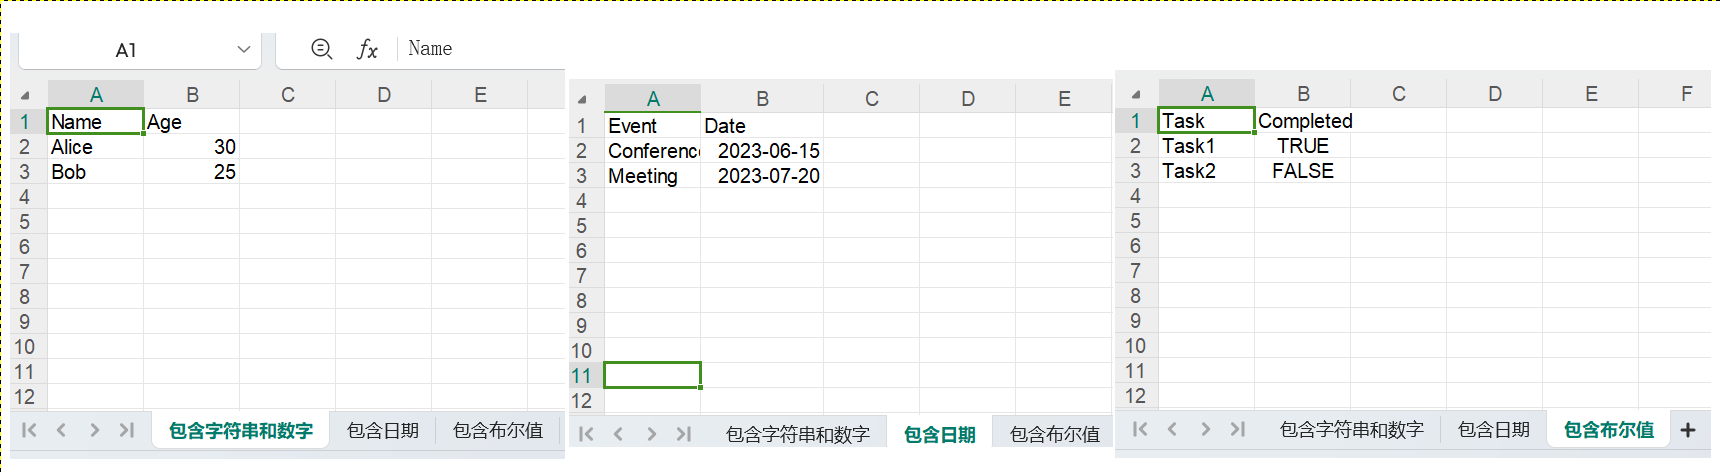
\includegraphics[width=0.8\textwidth]{part/自动化/办公自动化/pic/excel/数据类型转换结果演示.png}
        \caption{数据类型转换结果演示}
        \label{fig:数据类型转换结果演示}
\end{figure}

\begin{lstlisting}[style=demostyle,numbers=none]
Sheet1  包含字符串和数字 Data:
Name Age
Alice 30.0
Bob 25.0

Sheet2  包含日期 Data:
Event Date
Conference 2023-06-15
Meeting 2023-07-20

Sheet3  包含布尔值 Data:
Task Completed
Task1
Task2
\end{lstlisting}


\section{合并单元格}
\label{subsec:xlwt合并单元格}
\begin{lstlisting}[style=demostyle,numbers=none]
# 使用write_merge() 函数可以合并单元格
## write_merge(row1, row2, col1, col2, value, style)
## row1: 起始行
## row2: 结束行
## col1: 起始列
## col2: 结束列
## value: 写入的值
## style: 单元格样式
\end{lstlisting}

\begin{lstlisting}[style=pythonstyle,numbers=left]
import xlrd
import xlwt
from xlutils.copy import copy

# 打开现有的 Excel 文件
input_file = 'example.xls'
workbook = xlrd.open_workbook(input_file, formatting_info=True)
sheet = workbook.sheet_by_index(0)

# 创建一个新的工作簿，并将现有工作簿的内容复制到新的工作簿中
new_workbook = copy(workbook)
new_sheet = new_workbook.get_sheet(0)

# 合并单元格并设置内容
# 合并第2行第2列到第2行第4列的单元格（索引从0开始）
new_sheet.write_merge(1, 1, 1, 3, 'Merged Cell Content')

# 保存修改后的工作簿
output_file = 'merged_example.xls'
new_workbook.save(output_file)

print(f"合并单元格后的 Excel 文件已保存为 {output_file}")
\end{lstlisting}


\section{使用Excel函数}
\label{subsec:xlwt使用Excel函数}

\begin{lstlisting}[style=demostyle,numbers=none]
# 使用 xlwt.Formula() 函数可以在单元格中使用 Excel 函数
## 以下是一些常用的 Excel 函数
## SUM()：求和
## AVERAGE()：求平均值
## MAX()：求最大值
## MIN()：求最小值
## COUNT()：计数
## IF()：条件判断
## VLOOKUP()：垂直查找
## HLOOKUP()：水平查找
## CONCATENATE()：连接字符串
## LEFT()：提取字符串左边的字符
## RIGHT()：提取字符串右边的字符
## MID()：提取字符串中间的字符
## UPPER()：将字符串转换为大写
## LOWER()：将字符串转换为小写
## TRIM()：删除字符串两端的空格
## LEN()：计算字符串的长度
## DATE()：返回日期
## TIME()：返回时间
## NOW()：返回当前日期和时间
## RAND()：返回随机数
## PI()：返回圆周率
## SQRT()：求平方根
## POWER()：求幂
## LOG()：求对数
\end{lstlisting}

\begin{lstlisting}[style=pythonstyle,numbers=left]
import xlwt
from datetime import datetime

# 创建一个新的Excel工作簿
workbook = xlwt.Workbook()

# 数据样本
sample_data = [1, 2, 3, 4, 5]
lookup_data = [("A", 100), ("B", 200)]

# 演示SUM函数
sheet = workbook.add_sheet('演示SUM函数')
for row, value in enumerate(sample_data, start=1):
    sheet.write(row, 0, value)
sheet.write(0, 0, 'SUM')
sheet.write(0, 1, 'SUM(A2:A6)')
sheet.write(1, 2, xlwt.Formula('SUM(A2:A6)'))

# 演示AVERAGE函数
sheet = workbook.add_sheet('演示AVERAGE函数')
for row, value in enumerate(sample_data, start=1):
    sheet.write(row, 0, value)
sheet.write(0, 0, 'AVERAGE')
sheet.write(0, 1, 'AVERAGE(A2:A6)')
sheet.write(1, 2, xlwt.Formula('AVERAGE(A2:A6)'))

# 演示MAX函数
sheet = workbook.add_sheet('演示MAX函数')
for row, value in enumerate(sample_data, start=1):
    sheet.write(row, 0, value)
sheet.write(0, 0, 'MAX')
sheet.write(0, 1, 'MAX(A2:A6)')
sheet.write(1, 2, xlwt.Formula('MAX(A2:A6)'))

# 演示MIN函数
sheet = workbook.add_sheet('演示MIN函数')
for row, value in enumerate(sample_data, start=1):
    sheet.write(row, 0, value)
sheet.write(0, 0, 'MIN')
sheet.write(0, 1, 'MIN(A2:A6)')
sheet.write(1, 2, xlwt.Formula('MIN(A2:A6)'))

# 演示COUNT函数
sheet = workbook.add_sheet('演示COUNT函数')
for row, value in enumerate(sample_data, start=1):
    sheet.write(row, 0, value)
sheet.write(0, 0, 'COUNT')
sheet.write(0, 1, 'COUNT(A2:A6)')
sheet.write(1, 2, xlwt.Formula('COUNT(A2:A6)'))

# 演示IF函数
sheet = workbook.add_sheet('演示IF函数')
sheet.write(1, 0, 5)
sheet.write(0, 0, 'IF')
sheet.write(0, 1, 'IF(A2>10, "Greater than 10", "10 or less")')
sheet.write(1, 2, xlwt.Formula('IF(A2>10, "Greater than 10", "10 or less")'))

# 演示VLOOKUP函数
sheet = workbook.add_sheet('演示VLOOKUP函数')
for row, (key, value) in enumerate(lookup_data, start=6):
    sheet.write(row, 0, key)
    sheet.write(row, 1, value)
sheet.write(0, 0, 'VLOOKUP')
sheet.write(0, 1, 'VLOOKUP("B", $A$6:$B$7, 2, FALSE)')
sheet.write(1, 2, xlwt.Formula('VLOOKUP("B", $A$6:$B$7, 2, FALSE)'))

# 演示HLOOKUP函数
sheet = workbook.add_sheet('演示HLOOKUP函数')
for col, (key, value) in enumerate(lookup_data, start=6):
    sheet.write(0, col, key)
    sheet.write(1, col, value)
sheet.write(0, 0, 'HLOOKUP')
sheet.write(0, 1, 'HLOOKUP("B", $A$6:$B$7, 2, FALSE)')
sheet.write(2, 2, xlwt.Formula('HLOOKUP("B", $A$6:$B$7, 2, FALSE)'))

# 演示CONCATENATE函数
sheet = workbook.add_sheet('演示CONCATENATE函数')
sheet.write(1, 0, 'Hello')
sheet.write(1, 1, 'World')
sheet.write(0, 0, 'CONCATENATE')
sheet.write(0, 1, 'CONCATENATE(A2, " ", B2)')
sheet.write(1, 2, xlwt.Formula('CONCATENATE(A2, " ", B2)'))

# 演示LEFT函数
sheet = workbook.add_sheet('演示LEFT函数')
sheet.write(1, 0, 'Hello')
sheet.write(0, 0, 'LEFT')
sheet.write(0, 1, 'LEFT(A2, 3)')
sheet.write(1, 2, xlwt.Formula('LEFT(A2, 3)'))

# 演示RIGHT函数
sheet = workbook.add_sheet('演示RIGHT函数')
sheet.write(1, 0, 'Hello')
sheet.write(0, 0, 'RIGHT')
sheet.write(0, 1, 'RIGHT(A2, 3)')
sheet.write(1, 2, xlwt.Formula('RIGHT(A2, 3)'))

# 演示MID函数
sheet = workbook.add_sheet('演示MID函数')
sheet.write(1, 0, 'HelloWorld')
sheet.write(0, 0, 'MID')
sheet.write(0, 1, 'MID(A2, 2, 3)')
sheet.write(1, 2, xlwt.Formula('MID(A2, 2, 3)'))

# 演示UPPER函数
sheet = workbook.add_sheet('演示UPPER函数')
sheet.write(1, 0, 'hello')
sheet.write(0, 0, 'UPPER')
sheet.write(0, 1, 'UPPER(A2)')
sheet.write(1, 2, xlwt.Formula('UPPER(A2)'))

# 演示LOWER函数
sheet = workbook.add_sheet('演示LOWER函数')
sheet.write(1, 0, 'HELLO')
sheet.write(0, 0, 'LOWER')
sheet.write(0, 1, 'LOWER(A2)')
sheet.write(1, 2, xlwt.Formula('LOWER(A2)'))

# 演示TRIM函数
sheet = workbook.add_sheet('演示TRIM函数')
sheet.write(1, 0, '   Hello   ')
sheet.write(0, 0, 'TRIM')
sheet.write(0, 1, 'TRIM(A2)')
sheet.write(1, 2, xlwt.Formula('TRIM(A2)'))

# 演示LEN函数
sheet = workbook.add_sheet('演示LEN函数')
sheet.write(1, 0, 'Hello')
sheet.write(0, 0, 'LEN')
sheet.write(0, 1, 'LEN(A2)')
sheet.write(1, 2, xlwt.Formula('LEN(A2)'))

# 演示DATE函数
sheet = workbook.add_sheet('演示DATE函数')
sheet.write(0, 0, 'DATE')
sheet.write(0, 1, 'DATE(2023, 6, 15)')
sheet.write(1, 2, xlwt.Formula('DATE(2023, 6, 15)'))

# 演示TIME函数
sheet = workbook.add_sheet('演示TIME函数')
sheet.write(0, 0, 'TIME')
sheet.write(0, 1, 'TIME(12, 0, 0)')
sheet.write(1, 2, xlwt.Formula('TIME(12, 0, 0)'))

# 演示NOW函数
sheet = workbook.add_sheet('演示NOW函数')
sheet.write(0, 0, 'NOW')
sheet.write(0, 1, 'NOW()')
sheet.write(1, 2, xlwt.Formula('NOW()'))

# 演示RAND函数
sheet = workbook.add_sheet('演示RAND函数')
sheet.write(0, 0, 'RAND')
sheet.write(0, 1, 'RAND()')
sheet.write(1, 2, xlwt.Formula('RAND()'))

# # 演示RANDBETWEEN函数
# sheet = workbook.add_sheet('演示RANDBETWEEN函数')
# sheet.write(0, 0, 'RANDBETWEEN')
# sheet.write(0, 1, 'RANDBETWEEN(1, 100)')
# sheet.write(1, 2, xlwt.Formula('RANDBETWEEN(1, 100)'))

# 演示PI函数
sheet = workbook.add_sheet('演示PI函数')
sheet.write(0, 0, 'PI')
sheet.write(0, 1, 'PI()')
sheet.write(1, 2, xlwt.Formula('PI()'))

# 演示SQRT函数
sheet = workbook.add_sheet('演示SQRT函数')
sheet.write(1, 0, 16)
sheet.write(0, 0, 'SQRT')
sheet.write(0, 1, 'SQRT(A2)')
sheet.write(1, 2, xlwt.Formula('SQRT(A2)'))

# 演示POWER函数
sheet = workbook.add_sheet('演示POWER函数')
sheet.write(1, 0, 2)
sheet.write(0, 0, 'POWER')
sheet.write(0, 1, 'POWER(A2, 2)')
sheet.write(1, 2, xlwt.Formula('POWER(A2, 2)'))

# 演示LOG函数
sheet = workbook.add_sheet('演示LOG函数')
sheet.write(1, 0, 100)
sheet.write(0, 0, 'LOG')
sheet.write(0, 1, 'LOG(A2)')
sheet.write(1, 2, xlwt.Formula('LOG(A2)'))

# 保存工作簿
workbook.save('excel函数演示.xls')

import xlrd
# 打开已创建的Excel文件
workbook = xlrd.open_workbook('excel函数演示.xls')

# 读取每个工作表的数据
sheet_names = [
    '演示SUM函数', '演示AVERAGE函数', '演示MAX函数', '演示MIN函数', '演示COUNT函数',
    '演示IF函数', '演示VLOOKUP函数', '演示HLOOKUP函数', '演示CONCATENATE函数', '演示LEFT函数',
    '演示RIGHT函数', '演示MID函数', '演示UPPER函数', '演示LOWER函数', '演示TRIM函数',
    '演示LEN函数', '演示DATE函数', '演示TIME函数', '演示NOW函数', '演示RAND函数',
    '演示PI函数', '演示SQRT函数', '演示POWER函数', '演示LOG函数'
]

for sheet_name in sheet_names:
    sheet = workbook.sheet_by_name(sheet_name)
    print(f"\n{sheet_name} Data:")
    for row in range(sheet.nrows):
        for col in range(sheet.ncols):
            cell = sheet.cell(row, col)
            if cell.ctype == 2:  # xlrd.XL_CELL_NUMBER
                print(f"Number: {cell.value}", end=' ')
            elif cell.ctype == 3:  # xlrd.XL_CELL_DATE
                date_value = xlrd.xldate_as_tuple(cell.value, workbook.datemode)
                print(f"Date: {datetime(*date_value)}", end=' ')
            elif cell.ctype == 4:  # xlrd.XL_CELL_BOOLEAN
                print(f"Boolean: {cell.value}", end=' ')
            elif cell.ctype == 5:  # xlrd.XL_CELL_ERROR
                print(f"Error: {cell.value}", end=' ')
            elif cell.ctype == 6:  # xlrd.XL_CELL_FORMULA
                print(f"Formula: {cell.value}", end=' ')
            else:  # xlrd.XL_CELL_TEXT (1) or xlrd.XL_CELL_EMPTY (0)
                print(cell.value, end=' ')
        print()
\end{lstlisting}



\section{复制现有的Excel文件并添加新的数据}
\label{subsec:xlutils复制现有的Excel文件并添加新的数据}
\begin{lstlisting}[style=demostyle,numbers=none]
# xlutils 的函数
## copy() 复制工作簿
## add_sheet() 添加工作表
## save() 保存工作簿
\end{lstlisting}

\begin{lstlisting}[style=pythonstyle,numbers=left]
import xlrd
import xlwt
from xlutils.copy import copy

# 打开现有的 Excel 文件
input_file = 'excel/example.xls'
workbook = xlrd.open_workbook(input_file, formatting_info=True)
sheet = workbook.sheet_by_index(0)

# 创建一个新的工作簿，并将现有工作簿的内容复制到新的工作簿中
new_workbook = copy(workbook)
new_sheet = new_workbook.get_sheet(0)

# 在新的工作簿中添加新的数据
new_data = [
    ['Name', 'Age', 'City'],
    ['Alice', 30, 'New York'],
    ['Bob', 25, 'Los Angeles'],
    ['Charlie', 35, 'Chicago']
]

# 添加新的数据到现有工作表中
start_row = sheet.nrows  # 从现有数据的下一行开始添加新数据
for row_idx, row_data in enumerate(new_data, start=start_row):
    for col_idx, cell_value in enumerate(row_data):
        new_sheet.write(row_idx, col_idx, cell_value)

# 添加一个新的工作表
additional_sheet = new_workbook.add_sheet('NewDataSheet')

# 在新的工作表中添加数据
additional_data = [
    ['Product', 'Price', 'Quantity'],
    ['Apple', 1.2, 50],
    ['Banana', 0.5, 100],
    ['Cherry', 2.5, 200]
]

# 添加新的数据到新的工作表中
for row_idx, row_data in enumerate(additional_data):
    for col_idx, cell_value in enumerate(row_data):
        additional_sheet.write(row_idx, col_idx, cell_value)

# 保存新的工作簿
output_file = 'new_example_with_additional_sheet.xls'
new_workbook.save(output_file)

print(f"新的 Excel 文件已保存为 {output_file}")
\end{lstlisting}



\section{合并多个Excel文件}
\label{subsec:xlutils合并多个Excel文件}
\begin{lstlisting}[style=pythonstyle,numbers=left]
import xlrd
import xlwt
from xlutils.copy import copy

def read_excel_data(file_name):
    workbook = xlrd.open_workbook(file_name)
    sheet = workbook.sheet_by_index(0)
    data = []
    for row_idx in range(sheet.nrows):
        row_data = sheet.row_values(row_idx)
        data.append(row_data)
    return data

def write_data_to_sheet(sheet, data, start_row=0):
    for row_idx, row_data in enumerate(data, start=start_row):
        for col_idx, cell_value in enumerate(row_data):
            sheet.write(row_idx, col_idx, cell_value)

# 读取多个 Excel 文件
file_names = ['file1.xls', 'file2.xls', 'file3.xls']
all_data = []
for file_name in file_names:
    data = read_excel_data(file_name)
    all_data.append(data)

# 创建一个新的工作簿
new_workbook = xlwt.Workbook()
new_sheet = new_workbook.add_sheet('MergedData')

# 写入数据到新的工作表中
start_row = 0
for data in all_data:
    write_data_to_sheet(new_sheet, data, start_row)
    start_row += len(data)

# 保存新的工作簿
output_file = 'merged_example.xls'
new_workbook.save(output_file)

print(f"新的合并后的 Excel 文件已保存为 {output_file}")
\end{lstlisting}

\section{修改现有的Excel文件}
\label{subsec:xlutils修改现有的Excel文件}
\begin{lstlisting}[style=pythonstyle,numbers=left]
import xlrd
import xlwt
from xlutils.copy import copy

# 打开现有的 Excel 文件
input_file = 'excel/example.xls'
workbook = xlrd.open_workbook(input_file, formatting_info=True)
sheet = workbook.sheet_by_index(0)

# 创建一个新的工作簿，并将现有工作簿的内容复制到新的工作簿中
new_workbook = copy(workbook)
new_sheet = new_workbook.get_sheet(0)

# 修改现有的数据
# 例如，修改第1行第1列（索引从0开始）的数据为 'Modified'
new_sheet.write(0, 0, 'Modified')

# 添加新数据到现有的工作表中
new_data = [
    ['New Name', 'New Age', 'New City'],
    ['David', 40, 'San Francisco'],
    ['Eva', 28, 'Seattle']
]

# 确定从哪一行开始添加新数据
start_row = sheet.nrows  # 从现有数据的下一行开始添加新数据
for row_idx, row_data in enumerate(new_data, start=start_row):
    for col_idx, cell_value in enumerate(row_data):
        new_sheet.write(row_idx, col_idx, cell_value)

# 保存修改后的工作簿
output_file = 'modified_example.xls'
new_workbook.save(output_file)

print(f"修改后的 Excel 文件已保存为 {output_file}")
\end{lstlisting}
